\documentclass{article}
\usepackage{graphicx} % Required for inserting images
\usepackage[a4paper, total={6in, 10in}]{geometry}
\usepackage{hyperref}
\usepackage{amsmath}
\usepackage{amssymb}
\usepackage{bm}
\usepackage{pgfplots}
\usepackage{tikz}
\usepackage{float}
\pgfplotsset{width=10cm,compat=1.9}
\usepgfplotslibrary{external}
\usepgfplotslibrary{fillbetween}
\pgfplotsset{compat=1.18} % Ensure compatibility with your pgfplots version
\tikzexternalize

\title{Dayan and Abbott Notes}
\author{Rory Bedford}
\date{August 2024}

\begin{document}

\maketitle

These notes are written for the neuroscience reading group at the LMB, and are therefore aimed at biologists, with a less quantitative background. Some topics within Dayan and Abbott will be mathematically tricky for these readers, so my intention here is to give an overview of many of the topics covered to make things more digestible. Focus is therefore on understanding concepts broadly and how they relate to actual neurobiology, without getting too bogged down in derivations. That said, some familiarity with linear algebra, multivariate calculus and probability theory are still prerequisites for this. If you need a reference for these, I would highly recommend the first half of the textbook \href{https://mml-book.github.io/}{Mathematics for Machine Learning}. The appendix of Dayan and Abbott is also a fantastic resource.\\

The book is split into three main sections. In the first section, we look at how neurons encode information about the environment. In the second section, we look at biophysical models of neurons such as the Hodgkin-Huxley model, and work our way up to modelling biophysically plausible neural networks. In the final section, we look at learning, including mathematical models of plasticity, some basic reinforcement learning, and some Bayesian inference methods.\\

Note that my discussion for each chapter does not follow the material in the book in order but jumps around a little. I therefore reference the corresponding section in the book.

\section{Chapter 1 - Neural Encoding I}

In this chapter, we first look at neuron spike trains and firing rates, which are two different ways of thinking about a neuron's activity. We look at the relationship between these two forms, and how to convert between the two. We also have a first look at neural encoding, with neuron tuning curves and spike-triggered averages.

\subsection{Spike trains and firing rates}

Neurons fire action potentials at discrete points in time. If we measure a neuron's activity in a single trial, we end up with a list of times $t_i$ for $i = 1,2,...,n$ for n spikes, called a spike train. However, neurons don't work with infinite precision; there is some noise inherent in the timings of these action potentials. We therefore seek an alternate description of a neuron's activity that describes the \textit{rate} at which it is firing, not the exact times of its spikes. The spike-count rate is the neuron's firing rate measured across the entire trial. For a trial of length T:

\begin{equation*}
    r = \frac{n}{T}
\end{equation*}

The problem with this is that it doesn't account for variation of a neuron's firing rate within a trial, which is an important aspect of how neurons encode information. We therefore seek a firing rate \textit{function}, that varies with time, $r(t)$. This function is an abstraction that is a very useful way to think about neural activity given that spike trains are necessarily stochastic. We can think of it as being the same as the spike-count rate as above, but instead of considering the entire trial, we bin the trial into small windows of length $\Delta t$. We can then think of the function $r(t)$ as being the firing rate in the window $t$ to $t+\Delta t$, ie., the number of spikes in this window divided by $\Delta t$. This is not very useful if we are only considering one spike train, but if we perform the same recording across many trials, we can average their results to get a good description of a neuron's activity. Furthermore, the more trials we have, the smaller we can make the window $\Delta t$, and the more precise of firing rate function becomes.\\

\begin{figure}[ht]
\centering
    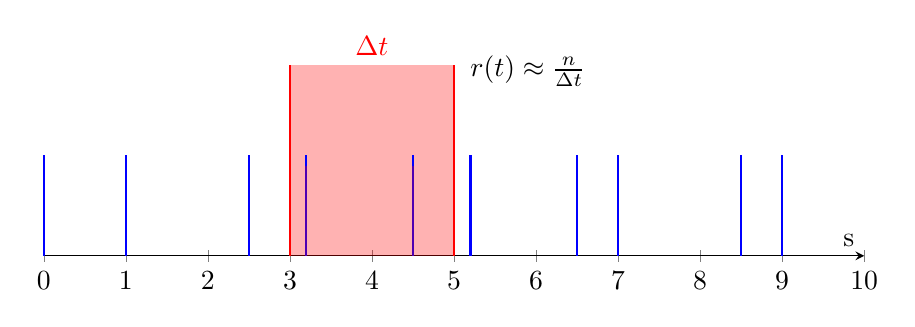
\begin{tikzpicture}
        \begin{axis}[
            width=12cm,
            height=4cm,
            axis y line=none,
            axis x line=middle,
            xmin=0, xmax=10,
            ymin=0, ymax=2,
            xlabel={s},
            clip=false
        ]
        
        % Spike train for a single neuron (small vertical lines)
        \addplot+[ycomb, thick, mark=|, mark size=2pt] 
            coordinates {
                (0, 1)
                (1, 1)
                (2.5, 1)
                (3.2, 1)
                (4.5, 1)
                (5.2, 1)
                (6.5, 1)
                (7, 1)
                (8.5, 1)
                (9, 1)
            };
        
        % Sliding window
        \fill[red, opacity=0.3] (axis cs:3,0) rectangle (axis cs:5,2);
        \draw[red, thick] (axis cs:3,0) -- (axis cs:3,2);
        \draw[red, thick] (axis cs:5,0) -- (axis cs:5,2);
        \node[red] at (axis cs:4,2.2) {$\Delta t$};

        \node[anchor=north] at (axis cs:5.9, 2.2) {$r(t) \approx \frac{n}{\Delta t}$};
        
        \end{axis}
    \end{tikzpicture}
\end{figure}

If we let the window size get infinitely small, then each window either catches a spike, or it doesn't. In this case, the firing rate is zero everywhere, apart from at the exact locations of a spike, at which it is infinite. The function that describes this is the dirac delta function $\delta (t)$. This function has the important property that it integrates to 1, and can therefore be used to 'pick out' values of a continuous function from inside an integral:

\begin{equation*}
    \int dt' \delta (t-t') f(t') = f(t)
\end{equation*}

We can now represent our spike train as a continuous function $\rho (t)$, rather than just a set of spike times, given by:

\begin{equation*}
    \rho (t) = \sum_{i=1}^n \delta(t-t_i)
\end{equation*}

For clarity, $\rho(t)$ is the particular function that we measure when recording a neuron's spiking activity. This is generated stochastically from the true underlying firing rate $r(t)$, which doesn't spike but gives a varying firing \textit{rate} over time.\\

We now need to look at how to convert between these two representations of a neuron's activity - ie, how to estimate $r(t)$ from a set of measured spike trains $\rho(t)$, and additionally, how to sample a spike train from a firing rate function.

\subsection{Spike train smoothing}

If we could record an infinite number of trials, then our simple window method above would converge to the true firing rate as the window size gets infinitely small. In practise, however, we generally need to estimate the firing rate from a finite number of trials. To do this, we smooth out our set of spike trains by performing a \textit{convolution} with a \textit{window} function $w(\tau)$. A convolution refers to the process of integrating our function of interest with a small sliding window function, sometimes called a kernel, as follows:\\

\begin{equation*}
    r(t) \approx \int_{- \infty}^{\infty} d\tau w(\tau) \rho(t-\tau)
\end{equation*}

If you think carefully about this equation, you see that at time t, we centre our window function at t, then compute the values of the window function at all neighbouring spikes, and add their values to give an estimate of the firing rate, as shown below. Also note that in practise, you can average this method over many trials where you have recorded the same neuron to get better results.\\

\begin{figure}[H]
    \centering
    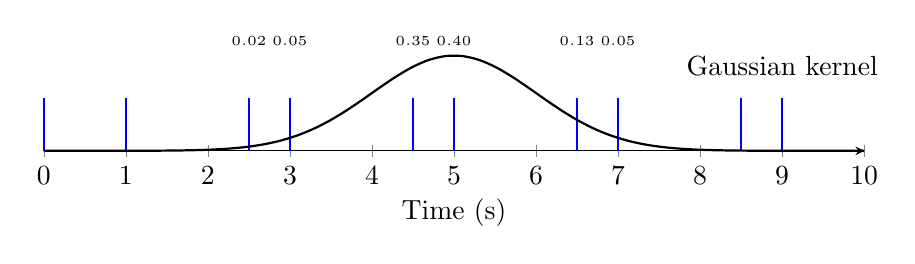
\begin{tikzpicture}
        \begin{axis}[
            width=12cm,
            height=4cm,
            xlabel={Time (s)},
            xlabel style={at={(axis description cs:0.5,-0.2)}, anchor=north},
            axis y line=none,
            axis x line=bottom,
            xmin=0, xmax=10,
            ymin=0, ymax=2,
            clip=false,
            domain=0:10
        ]
        
        % Spike train for a single neuron (small vertical lines)
        \addplot+[ycomb, thick, mark=|, mark size=2pt] 
            coordinates {
                (0, 0.5)
                (1, 0.5)
                (2.5, 0.5)
                (3, 0.5)
                (4.5, 0.5)
                (5, 0.5)
                (6.5, 0.5)
                (7, 0.5)
                (8.5, 0.5)
                (9, 0.5)
            };
        
        % Gaussian kernel
        \addplot[
            domain=0:10,
            samples=100,
            thick,
            black,
            samples=50,
            unbounded coords=jump,
            smooth
        ] {exp(-((x-5)^2)/(2*1^2))}; % Gaussian function with mean 5 and stddev 1

        \node[anchor=north] at (axis cs:9, 1.1) {Gaussian kernel};

        \node[anchor=south, font=\tiny] at (axis cs:2.5, 1) {$0.02$};
        \node[anchor=south, font=\tiny] at (axis cs:3, 1) {$0.05$};
        \node[anchor=south, font=\tiny] at (axis cs:4.5, 1) {$0.35$};
        \node[anchor=south, font=\tiny] at (axis cs:5, 1) {$0.40$};
        \node[anchor=south, font=\tiny] at (axis cs:6.5, 1) {$0.13$};
        \node[anchor=south, font=\tiny] at (axis cs:7, 1) {$0.05$};
        
        \end{axis}
    
    \end{tikzpicture}


    \begin{align*}
        r(5) &\approx 0.02 + 0.05 + 0.35 + 0.40 + 0.13 + 0.05\\
        &\approx 1 \text{Hz}
    \end{align*}
\end{figure}

Since our Gaussian window function varies smoothly, the effect is to smooth out the firing rate function. Smoothing the firing rate captures the fact that a spike train is generated stochastically from the firing rate - the smoother we make it, by widening the window width, the more we get a general rate, and the less the precise spike timings matter. The effects of using different window functions is shown in Figure 1.4 in the book.

\subsection{Poisson processes}

Having seen how we can estimate the firing rate from a set of recorded spike trains, we also want to consider how spike trains are actually generated from a given firing rate function.\\

First of all, note that we can easily calculate the mean number of spikes in a trial, as follows:

\begin{align*}
    \mathbb{E} [N] &= \int_0^T r(t)dt\\
    &= rT \text{ if r constant}
\end{align*}

However, this tells us nothing about the distribution of spikes around this mean rate. The most basic way to generate spikes is to use a Poisson process. Consider the probability of there being a spike in the window $t$ to $t+\Delta t$. As $\Delta t \to 0$, the probability of there being 2 or more spikes in this box falls to 0, so we only need to consider the possibility of there being 0 or 1 spikes in this box. This is just a coin flip, or Bernoulli trial, with the probability of there being a spike being given by $P(\text{spike})=r(t)\Delta t$. Computationally, you could simulate a spike train by splitting your trial into a finite set of small boxes of size $\Delta t$, and putting a spike in each box with this probability.\\

In the case of a homogeneous firing rate - that is, one that is constant for the whole trial, we can say a bit more about the distribution of the number of spikes in a trial. This is done by counting all the different ways we can get n spikes in a finite set of boxes in a trial using combinatorics, and adding their probabilities, then letting our box sizes tend to zero, while using something called Sterling's approximation to give the following nice result:

\begin{equation*}
    P[N=n] = \frac{(rT)^n}{n!} \exp(-rT)
\end{equation*}

Which is the Poisson distribution with mean $rT$.\\

An issue with this simplified model is that we assume the probabilities of a spike being in any bin is independent of the probability of a spike being in any other bin. This is obviously false, and the most major way this is violated is due to a neuron's refractory period - that is, if it spikes, the immediately following bins are extremely unlikely to also spike, regardless of how high the firing rate is. More complex models are able to incorporate a refractory period - in particular, the book discusses methods that sample interspike intervals to generate spike trains. For the homogeneous poisson process, the interspike interval follows an exponential distribution (the derivation in the book is quite straightforward), but this can be modified to a gamma distribution, which can make it almost impossible for a neuron to spike in the refractory period following a different spike.

\subsection{Tuning curves}

So far, we've only considered a neuron's activity in isolation. We now being our exploration of how a neuron can encode information about a stimulus. Chapter 1 really only makes a cursory first pass at this, but it gives a good flavour of what's to come.\\

First of all we consider the concept of a tuning curve. Tuning curves capture the relationship between the values of a stimulus and the mean firing rate of a neuron that encodes this stimulus. They are therefore a useful way of characterising the selectivity of a neuron to sensory information.\\

Here, we make the simplification that a neuron only encodes information via its mean firing rate - ie, there is no temporal encoding of information, only $<r>$ matters. We consider a parameterised stimulus $s$. For example, the book shows a moving bar in Figure 1.5(A) with its angle of rotation as the parameter of the stimulus. We then simply hold this parameter constant and record the neuron's activity, and calculate its mean firing rate over a trial of given duration. We can vary the value of the parameter(s) across different trials, to build up a picture of how the mean firing rate varies as the stimulus varies. We can then perform any type of curve fitting we want to this dataset to obtain a tuning curve.\\

This is a useful but slightly limited thing to do. It tells us nothing about how a neuron's activity varies around its mean firing rate. Some of this information could be very useful - for example, think of a neuron in an oscillatory system; information could certainly be encoded in the frequency of its response. A tuning curve would assign the same response to neurons with wildly different oscillating frequencies and would completely miss this encoding. It also can't account for temporal changes in parameters of the stimulus during a trial. Furthermore, many natural stimuli would be almost impossible to effectively parameterise - it therefore only really applies to simple stimuli such as gratings for vision.

\subsection{Spike-triggered average}

Another fundamental concept is the spike-triggered average. This is a way of characterising what type of stimulus is most likely to drive a spike. At present we will just define what a spike-triggered average actually is; justification for why this is useful comes in the next chapter when we study receptive fields, which essentially encompass these ideas and tuning curves.\\

At present, we once again have a parameterised stimulus, which we now allow to vary with with time, $s(t)$. We won't worry exactly how it varies - this will be considered in the next chapter. All we need to do to compute the spike-triggered average, is to record a neuron's activity alongside this varying stimulus in a trial. We then pick a window of finite time, and take the mean of the changing stimulus across all the windows preceding all spikes in the recording. We then average this result over any trials. This is described by the following equation:

\begin{equation*}
    C(\tau) = \langle\frac{1}{n}\sum_{i=1}^n s(t_i-\tau)\rangle
\end{equation*}

Equation (1.20) also covers the integral forms of this equation in terms of $\rho(t)$ and $r(t)$. It's actually really useful to look at these to check your understanding of our previous discussion on firing rates vs spike trains. Below also shows a visual representation of the spike-triggered average. All we do is take the stimulus in the windows preceding each spike, as shaded, and average them, to obtain $C(\tau)$.\\

\begin{figure}[H]
    \centering
    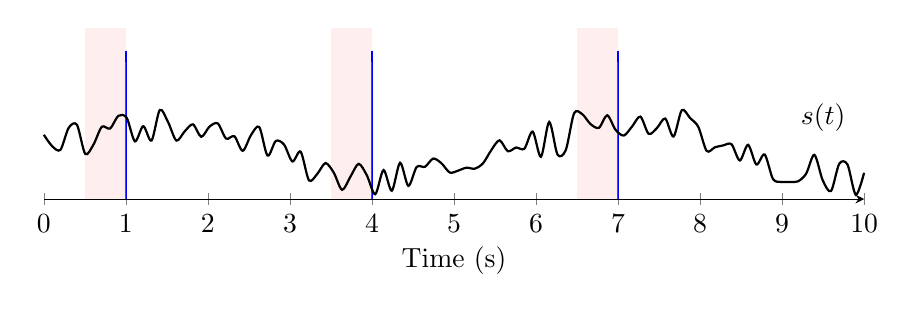
\begin{tikzpicture}
        % Define some colors for the stimulus and STA window
        \definecolor{stimuluscolor}{RGB}{150, 150, 255}
        \definecolor{stawindowcolor}{RGB}{255, 200, 200}
        
        \begin{axis}[
            width=12cm,
            height=4cm,
            xlabel={Time (s)},
            xlabel style={at={(axis description cs:0.5,-0.2)}, anchor=north},
            axis y line=none,
            axis x line=bottom,
            xmin=0, xmax=10,
            ymin=0, ymax=2,
            clip=false,
            domain=0:10
        ]

        % Spike train for a single neuron (small vertical lines)
        \addplot+[ycomb, thick, mark=|, mark size=2pt, color=blue] 
            coordinates {
                (1, 1.5)
                (4, 1.5)
                (7, 1.5)
            };

        % Shaded STA windows preceding each spike
        \foreach \x in {1, 4, 7} {
            \addplot [
                domain=\x-0.5:\x,
                samples=2,
                fill=stawindowcolor,
                fill opacity=0.3,
                draw=none
            ] {1.8} \closedcycle;
        }

        \addplot[
            domain=0:10,
            samples=100,
            thick,
            black,
            smooth
        ] {0.5 + 0.3 * sin(2*pi*10*x) + 0.2 * rand};

        \node[anchor=north] at (axis cs:9.5, 1.1) {$s(t)$};

        \end{axis}
    \end{tikzpicture}

\end{figure}

\section{Chapter 2 - Neural Encoding II}

In this chapter, we study neuron receptive fields and reverse-correlation techniques in detail. That is, we build models that can predict a neuron's activity given an arbitrary time-varying stimulus. These models work well for neurons in the early visual system, which is therefore discussed in detail. In the notes, I try to simplify the explanation of what reverse-correlation techniques are, but do not delve into all the examples of different types of receptive fields given in the notes, as the book describes these far better than I could in the notes.

\subsection{Correlation functions}

Before discussing reverse-correlation techniques, we need to briefly clarify some concepts from chapter 1.\\

To measure how much two functions correlate, we can multiply them and integrate over all of time. If both functions correlate, then we expect this integral to be positive, since when one function is positive, we expect the other function to also be positive, so they multiply to a positive number, and when one function is negative, we expect the other function to be negative, so they also multiply to give a positive. If this integral is negative, it means that on average the functions have opposing signs, and if the integral is zero, then they are uncorrelated - the value of one function tells us nothing about the value of the other function.\\

Say we want to compute how much the firing rate of a neuron correlates with a stimulus over the course of a trial. We are interested in the correlation of the neuron's activity with the stimulus at the same point in time, but also the correlation of the firing rate with values of the stimulus preceding the neuron's activity, since the neuron is influenced by the stimulus over a window of time prior to it responding. Therefore, we perform this correlation over successive shifts of the stimulus in time, and record the value as a function of this shift, rather than a single value, like so:

\begin{equation*}
    Q_{rs}(\tau) = \frac{1}{T} \int_0^Tdt \text{r}(t)s(t+\tau)
\end{equation*}

\begin{figure}[H]
    \centering
    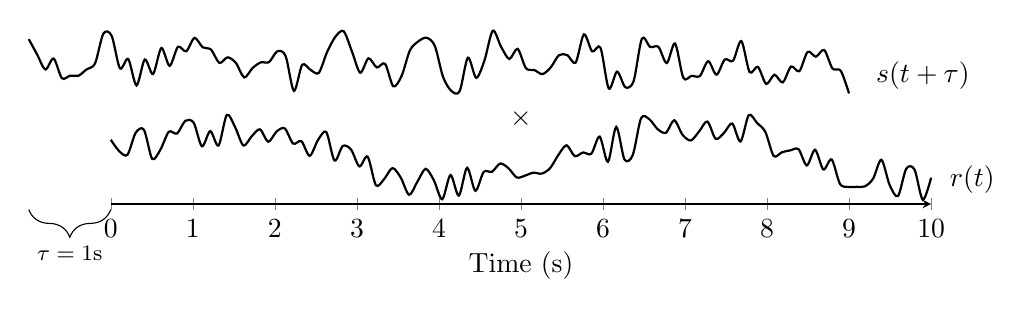
\begin{tikzpicture}
        % Define some colors for the stimulus and STA window
        \definecolor{stimuluscolor}{RGB}{150, 150, 255}
        \definecolor{stawindowcolor}{RGB}{255, 200, 200}
        
        \begin{axis}[
            width=12cm,
            height=4cm,
            xlabel={Time (s)},
            xlabel style={at={(axis description cs:0.5,-0.2)}, anchor=north},
            axis y line=none,
            axis x line=bottom,
            xmin=0, xmax=10,
            ymin=0, ymax=2,
            clip=false,
            domain=0:10
        ]

        \addplot[
            domain=0:10,
            samples=100,
            thick,
            black,
            smooth
        ] {0.5 + 0.3 * sin(2*pi*10*x) + 0.2 * rand};

        \addplot[
            domain=-1:9,
            samples=100,
            thick,
            black,
            smooth
        ] {1.5 + 0.15 * cos(15*pi*8*(x+1)) + 0.2 * rand};

        \node[anchor=north] at (axis cs:9.9, 1.6) {$s(t+\tau)$};
        \node[anchor=north] at (axis cs:10.5, 0.5) {$r(t)$};
        \node[anchor=north] at (axis cs:5, 1.1) {$\times$};
        
        % Add a curly bracket for displacement
        \draw[decorate,decoration={brace,amplitude=10pt,mirror,raise=2pt},yshift=0pt] 
            (axis cs:-1, 0) -- (axis cs:0, 0) node[midway,yshift=-18pt]{\footnotesize $\tau=1$s};

        \end{axis}
    \end{tikzpicture}

\end{figure}

We note the relationship here to the spike-triggered average. For the spike-triggered average, we average the stimulus in a window preceding each spike. Here, we average the stimulus preceding the firing rate, weighted by the firing rate. You see that they are essentially equivalent, since the firing rate is what underlies all spike trains. The only differences are that one is normalised by time, and the other by spike count, and also, that the shift $\tau$ is defined the other way around.\\

Rewriting the spike-triggered average in integral form (recalling that $\rho$ rewrites a spike train as a continuous function):

\begin{align*}
    C(\tau) =& \frac{1}{\langle n \rangle} \int_0^Tdt \langle \rho(t)\rangle s(t-\tau)\\
    =& \frac{1}{\langle n \rangle} \int_0^Tdt \text{r}(t) s(t-\tau)\\
    =& \frac{1}{\langle r \rangle} Q_{rs}(-\tau)
\end{align*}

It is also useful to define the stimulus autocorrelation function, which is the correlation of the stimulus with itself:

\begin{equation*}
    Q_{ss}(\tau) = \int_0^T dt s(t) s(t+\tau)
\end{equation*}

The following graph shows how we shift the function, multiply it by itself, and integrate over time.\\

\begin{figure}[H]
    \centering
    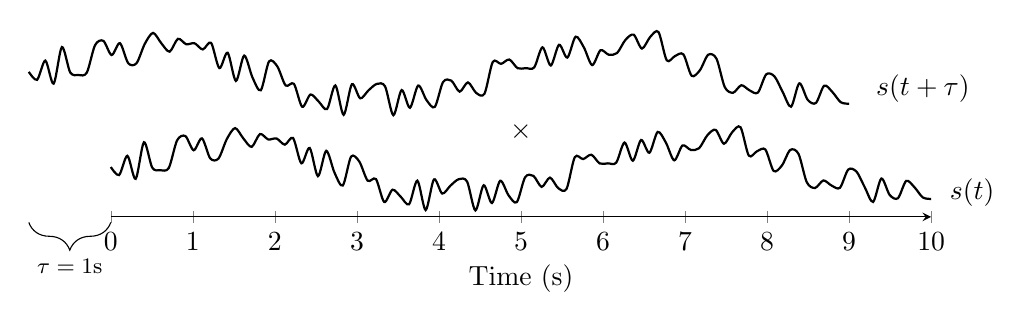
\begin{tikzpicture}
        % Define some colors for the stimulus and STA window
        \definecolor{stimuluscolor}{RGB}{150, 150, 255}
        \definecolor{stawindowcolor}{RGB}{255, 200, 200}
        
        \begin{axis}[
            width=12cm,
            height=4cm,
            xlabel={Time (s)},
            xlabel style={at={(axis description cs:0.5,-0.2)}, anchor=north},
            axis y line=none,
            axis x line=bottom,
            xmin=0, xmax=10,
            ymin=0, ymax=2,
            clip=false,
            domain=0:10
        ]

        \pgfmathsetseed{1234}
        \addplot[
            domain=0:10,
            samples=100,
            thick,
            black,
            smooth
        ] {0.5 + 0.3 * sin(2*pi*10*x) + 0.2 * rand};

        \pgfmathsetseed{1234}
        \addplot[
            domain=-1:9,
            samples=100,
            thick,
            black,
            smooth
        ] {1.5 + 0.3 * sin(2*pi*10*(x+1)) + 0.2 * rand};

        \node[anchor=north] at (axis cs:9.9, 1.6) {$s(t+\tau)$};
        \node[anchor=north] at (axis cs:10.5, 0.5) {$s(t)$};
        \node[anchor=north] at (axis cs:5, 1.1) {$\times$};
        
        % Add a curly bracket for displacement
        \draw[decorate,decoration={brace,amplitude=10pt,mirror,raise=2pt},yshift=0pt] 
            (axis cs:-1, 0) -- (axis cs:0, 0) node[midway,yshift=-18pt]{\footnotesize $\tau=1$s};

        \end{axis}
    \end{tikzpicture}

\end{figure}

Of particular importance is a white noise stimulus. This is a stimulus that is completely uncorrelated with itself - knowing its value at one time point tells you nothing about its value at any other timepoint. Its autocorrelation function is therefore zero for almost all values of $\tau$ - except for at zero, where the integral actually blows up to infinity. We represent this with a dirac delta function, which we met when studying spike trains. This is a standard result in signal processing, but understanding it fully requires diving into Fourier analysis, which we don't want to do now, so we just state that the following is the autocorrelation function for a white noise stimulus, where $\sigma_s$ is the signal's power:

\begin{equation*}
    Q_{ss}(\tau) = \sigma_s^2 \delta(\tau)
\end{equation*}

\subsection{Reverse-correlation methods}

We now have the correct toolkit to start studying how to predict a neuron's activity given the values of a stimulus that changes over time. This is actually a regression problem, and we will look at what amounts to linear regression. In regular linear regression, you have a finite set of input vectors and target values $\{(\bm{x}_i, y_i) | i=1:n\}$. We want to find a weight vector $\bm{w}$ and bias $b$ that can be used to estimate the target from an unseen input vector as follows:

\begin{equation*}
    y \approx \bm{w}^T\bm{x} + b
\end{equation*}

The solution will only ever be approximate as we assume there to be Gaussian noise added to all measurements. We solve this by minimising the least squares error on our available data:

\begin{equation*}
    \bm{w}, b = \text{argmin}_{\bm{w},b} \sum_{i=1}^n (y_i - \bm{w}^T\bm{x}_i - b)^2
\end{equation*}

In the special case of whitened input data, which means that the input data has been normalised to have zero mean and covariance proportional to the identity matrix, the solution to this problem is given by:

\begin{align*}
    \bm{w} &= \frac{1}{n\sigma^2} \sum_{i=1}^n y_i \bm{x}_i\\
    b &= \frac{1}{n} \sum_{i=1}^n y_i
\end{align*}

Where $\sigma^2$ is the input data variance. (Note this is also tractable in the case of non-whitened data, which is the solution you will typically see in textbooks. Also note that typically 'whitened' also means $\sigma^2=1$ but I keep a symmetric variance here for analogy later.)\\

Now, in the case of neural encoding, we want to calculate the firing rate of a neuron at time t, $r(t)$, given the value of the stimulus in a window leading up to the time t, as follows:\\

\begin{figure}[H]
    \centering
    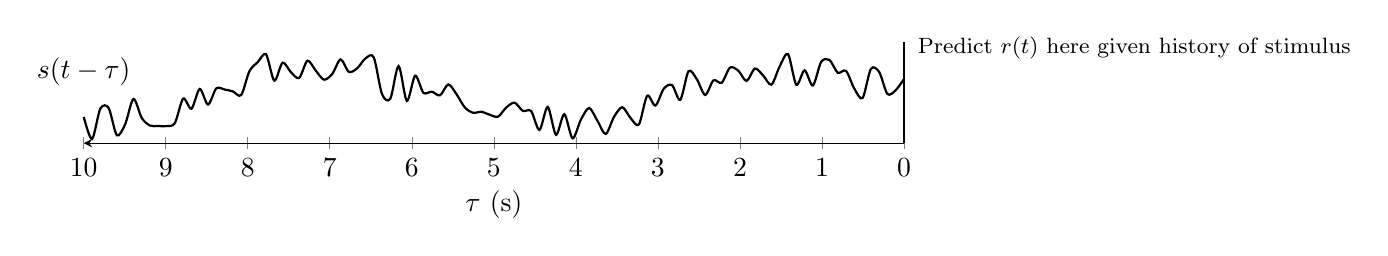
\begin{tikzpicture}
        % Define some colors for the stimulus and STA window
        \definecolor{stimuluscolor}{RGB}{150, 150, 255}
        \definecolor{stawindowcolor}{RGB}{255, 200, 200}
        
        \begin{axis}[
            width=12cm,
            height=4cm,
            xlabel={$\tau$ (s)},
            xlabel style={at={(axis description cs:0.5,-0.2)}, anchor=north},
            axis y line=none,
            axis x line=bottom,
            xmin=0, xmax=10,
            ymin=0, ymax=2,
            clip=false,
            domain=0:10,
            x dir=reverse,
        ]

        \addplot[
            domain=0:10,
            samples=100,
            thick,
            black,
            smooth
        ] {0.5 + 0.3 * sin(2*pi*10*x) + 0.2 * rand};

        \node[anchor=north] at (axis cs:10, 1) {$s(t-\tau)$};

        \addplot+[ycomb, thick, mark=|, mark size=2pt, color=black] 
            coordinates {
                (0, 1)
            };
            \node at (axis cs:-0.05,1) [anchor=west, font=\footnotesize] {Predict $r(t)$ here given history of stimulus};

        
        \end{axis}
    \end{tikzpicture}

\end{figure}

Now, the best way to think about this problem is that the values of $s(t-\tau)$ in the window leading up to the time $t$ at which we want to predict the firing rate form the input vector for our linear regression, and $r(t)$ itself forms the target scalar. It may seem strange that we are referring to a function as a vector, however, this is actually very common. You should think of the vector $\bm{s}$ as being labelled by a continuous variable $\tau$, so it has continuously many components, compared to a column vector $\bm{x}$ which is discretely labelled. Additionally, $t$ takes the place of the index $i$ in the linear regression problem - where before, we had a discrete number of input vectors and targets, here we use the continuously indexed $r(t)$ as targets with the stimulus values in the window leading up to $t$ as the input vectors. So there are two senses in which we have extended linear regression to a continuous domain.\\

\begin{align*}
    \bm{x}_i &\rightarrow s(t-\tau)\\
    y_i &\rightarrow r(t)\\
    i &\rightarrow t\\
    \tau &\rightarrow \text{column index of } \bm{x}\\
\end{align*}

Many equations from the discrete case can be translated into the continuous case by replacing the appropriate sum over the vector components with an integral over the corresponding function's continuous label. Therefore, a dot product between two vectors becomes an integral of the product of the two functions. We therefore replace the weight matrix $\bm{w}$ with a function $D(\tau)$. This is referred to as the filter.

\begin{align*}
    D(\tau) &\rightarrow \bm{w}\\
    r_0 &\rightarrow b
\end{align*}

The linear equation we want to solve for therefore becomes the integral of the weight function times the stimulus function, integrated over the the stimulus' history:

\begin{equation*}
    r_{\text{est}}(t) = r_0 + \int_0^\infty d\tau D(\tau)s(t-\tau)
\end{equation*}

And our training dataset becomes the continuous set of all such $(r(t), s(t-\tau))$ pairs present in the recording. Just like before, we minimise the least squares error on the training dataset, which takes the following form:

\begin{equation*}
    E = \frac{1}{T} \int_0^T dt (r(t) - r_{\text{est}}(t))^2
\end{equation*}

Note also how the normalising constant has changed from the number of datapoints $N$ to the continuous length of the trial $T$.\\

Minimising this equation properly is non-trivial, and requires something called a functional derivative from a subject called the calculus of variations. However, in this case (and definitely don't assume this will always be true!), our solution holds in direct analogy with standard linear regression for the specific case of a white noise stimulus. Previously, we whitened our input data, so that the vectors $\bm{x}$ have zero mean and symmetric variance. Here, we use a white-noise stimulus, which is the continuous analog of this, giving the solution:

\begin{align*}
    D(\tau) &= \frac{1}{T\sigma_s^2} \int_0^T dt \text{r}(t) s(t-\tau)\\
    r_0 &= \frac{1}{T} \int_0^T dt \text{r}(t)
\end{align*}

Now, this equation should look familiar. It is in fact, almost exactly the spike-triggered average, with slightly different normalising constants. Substituting these gives us:

\begin{equation*}
    D(\tau) = \frac{\langle r \rangle C(\tau)}{\sigma_s^2}
\end{equation*}

This is exactly why the spike-triggered average is a useful thing to calculate. It tells us the optimal linear filter for predicting a neuron's activity from a stimulus.\\

\begin{figure}[H]
    \centering
    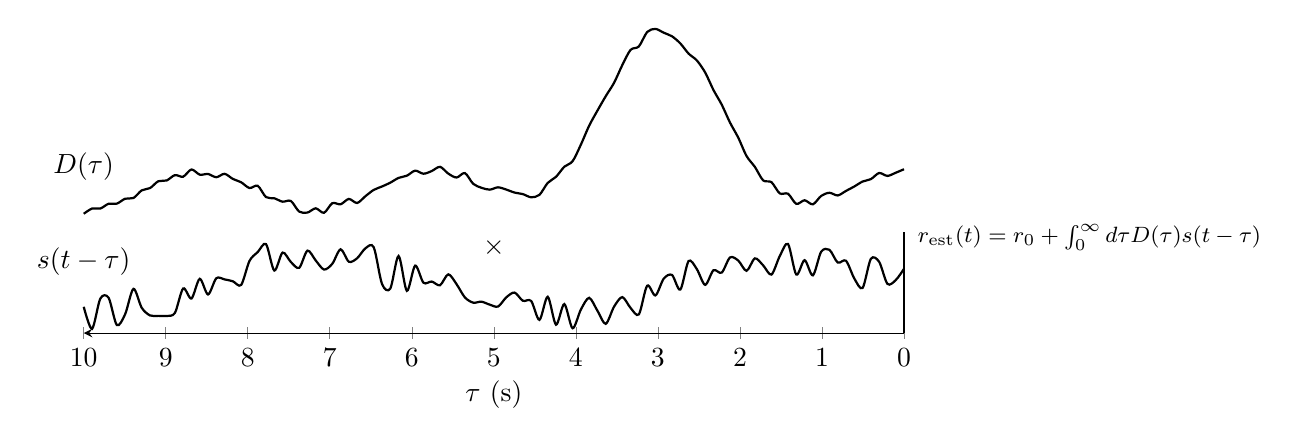
\begin{tikzpicture}
        % Define some colors for the stimulus and STA window
        \definecolor{stimuluscolor}{RGB}{150, 150, 255}
        \definecolor{stawindowcolor}{RGB}{255, 200, 200}
        
        \begin{axis}[
            width=12cm,
            height=4cm,
            xlabel={$\tau$ (s)},
            xlabel style={at={(axis description cs:0.5,-0.2)}, anchor=north},
            axis y line=none,
            axis x line=bottom,
            xmin=0, xmax=10,
            ymin=0, ymax=2,
            clip=false,
            domain=0:10,
            x dir=reverse,
        ]

        \addplot[
            domain=0:10,
            samples=100,
            thick,
            black,
            smooth
        ] {0.5 + 0.3 * sin(2*pi*10*x) + 0.2 * rand};

        \addplot[
            domain=0:10,
            samples=100,
            thick,
            black,
            smooth
        ] {1.5 + 0.2 * cos(2*pi*20*x) + 0.05 * rand + 1.5 * exp(-(x-3)^2)};

        \node[anchor=north] at (axis cs:10, 1) {$s(t-\tau)$};
        \node[anchor=north] at (axis cs:10, 2) {$D(\tau)$};
        \node[anchor=north] at (axis cs:5, 1.1) {$\times$};

        \addplot+[ycomb, thick, mark=|, mark size=2pt, color=black] 
            coordinates {
                (0, 1)
            };
        \node at (axis cs:-0.05,1) [anchor=west, font=\footnotesize] {$r_{\text{est}}(t) = r_0 + \int_0^\infty d\tau D(\tau)s(t-\tau)$};

        
        \end{axis}
    \end{tikzpicture}

\end{figure}

The case of a non-whitened stimulus is more complex, and requires the use of Fourier analysis to solve properly, which is beyond the scope of these notes. However, it is worth mentioning why a whiten-noise stimulus makes this problem easier to solve. In the non-whitened case, variations of the stimulus in a window leading up to the time at which we want to predict $r(t)$ affect not only $r(t)$, but also each other. Therefore, solving the problem requires completely disentangling the internal correlations in the stimulus, so we can see what directly caused the response, rather than what may have indirectly caused the response through affecting the stimulus value elsewhere.\\

It's also important to discuss the limitations associated with a linear model. A linear model assumes the response of a neuron is proportional to the amount of overlap its actual stimulus has with its most effective stimulus. We give here a graphical demonstration of what this entails.\\

\begin{figure}[H]
    \centering
    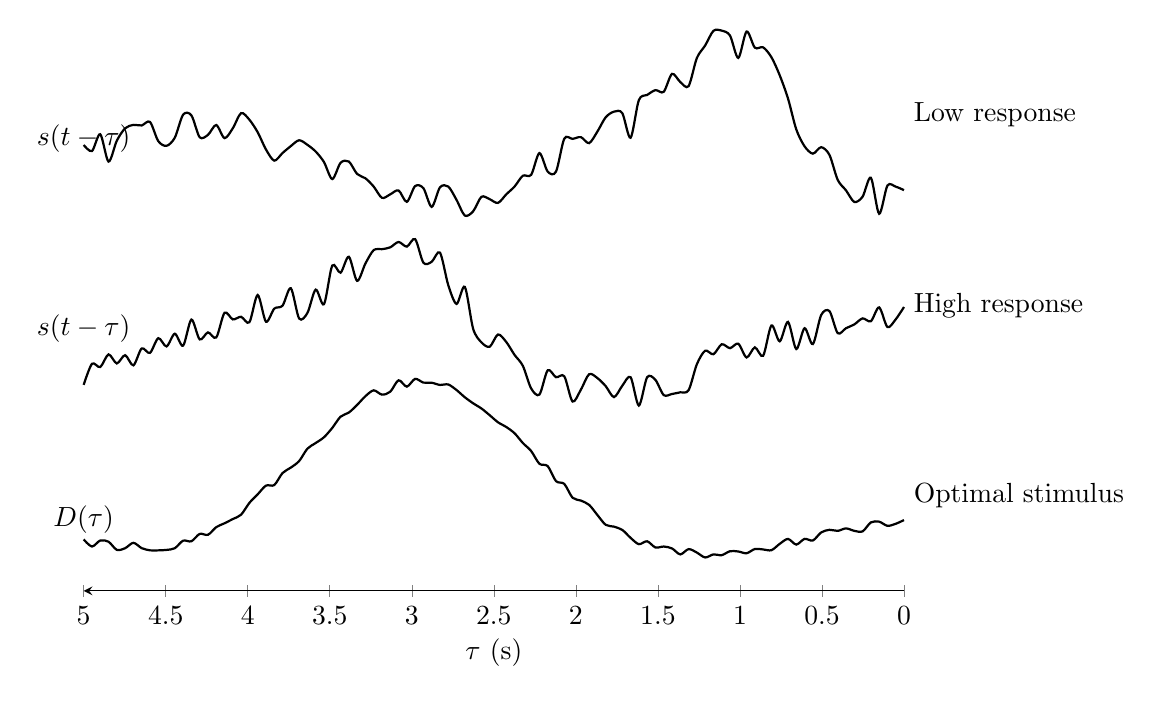
\begin{tikzpicture}
        % Define some colors for the stimulus and STA window
        \definecolor{stimuluscolor}{RGB}{150, 150, 255}
        \definecolor{stawindowcolor}{RGB}{255, 200, 200}
        
        \begin{axis}[
            width=12cm,
            height=4cm,
            xlabel={$\tau$ (s)},
            xlabel style={at={(axis description cs:0.5,-0.2)}, anchor=north},
            axis y line=none,
            axis x line=bottom,
            xmin=0, xmax=5,
            ymin=0, ymax=2,
            clip=false,
            domain=0:5,
            x dir=reverse,
        ]

        \addplot[
            domain=0:5,
            samples=100,
            thick,
            black,
            smooth
        ] {0.5 + 0.2 * cos(2*pi*20*x) + 0.05 * rand + 1.5 * exp(-(x-3)^2)};

        \node[anchor=north] at (axis cs:5, 1) {$D(\tau)$};
        \node[anchor=west] at (axis cs:0, 1) {Optimal stimulus};

        \addplot[
            domain=0:5,
            samples=100,
            thick,
            black,
            smooth
        ] {2.5 + 0.4 * cos(2*pi*15*x) + 0.2 * rand + 1 * exp(-(x-3)^2/0.25)};

        \node[anchor=north] at (axis cs:5, 3) {$s(t-\tau)$};
        \node[anchor=west] at (axis cs:0, 3) {High response};

        \addplot[
            domain=0:5,
            samples=100,
            thick,
            black,
            smooth
        ] {4.5 - 0.4 * cos(2*pi*20*x) + 0.2 * rand + 1 * exp(-(x-1)^2/0.2)};

        \node[anchor=north] at (axis cs:5, 5) {$s(t-\tau)$};
        \node[anchor=west] at (axis cs:0, 5) {Low response};

        \end{axis}
    \end{tikzpicture}

\end{figure}

We see here that we predict a low response when the stimulus doesn't overlap much with the optimal response. There is in fact no reason apriori to assume this is the case. Later in the chapter, we discuss complex neurons which can have, for example, position-invariant responses to a visual stimulus. A linear model could not capture such a neuron's behaviour: shifting the stimulus in the visual field would cause it to no longer overlap with the optimal stimulus, and hence a linear model would predict a low response.\\

We make a quick note here on non-linear models. Do not worry about this too much if you've found this material difficult. The book mentions 3 ways of extending this approach to non-linear models. First of all, it mentions the Volterra/Wiener expansion. This is the functional equivalent of the Taylor series, which allows you to approximate many functions with a polynomial. Including further terms in this expansion is therefore exactly equivalent to do higher-order polynomial regression\\

They also discuss using static non-linearities. This is where we compute exactly the same linear filter as before, but pass the output through a pointwise non-linear function, which is optimised to further improve our results. This is different to the full non-linear approach, because the full non-linear approach can model how arbitrary stimuli can affect the response. In the diagram above, both arbitrary stimuli could give high responses, for example, whereas in the static non-linearity approach (assuming a monotonic non-linearity), these would still necessarily get mapped to low and high responses respectively, its just the amount by which the neuron responds is modified in a non-linear way. Finally, the book mentions the use of a non-linearity inside the integral, and in particular, using the response tuning curve for this, so you integrate its static response over time, and develop an optimal linear kernel for that.\\

Its worth mentioning that many modern approaches to neural encoding will use arbitrarily complex, non-linear models such as deep-learning based approaches. For example, many deeper neurons in the visual system can be modelled well by CNNs.

\subsection{Receptive fields}

Most of this chapter is concerned with the early visual system. This is because these neurons can be well described by linear models, and are well studied.\\

So far, we have only studied stimuli that take scalar values. This could include, for example, the total intensity of light in a room. Most real-world stimuli are more complex than this, however, so we need to describe them in more complex ways. A natural extension would be to consider vector-valued stimuli. In this chapter, however, since we are studying the visual system, we actually consider stimuli that vary over a 2D plane, such as a 2D image. Such stimuli can be described by their value not just over time, but over the x-,y-axes, like $s(x,y,t)$. Fortunately, all the results from before transfer very easily to this case. For example, the spike-triggered average is defined:

\begin{equation*}
    C(x,y,\tau) = \frac{1}{\langle n \rangle} \left \langle \sum_{i=1}^n s(x,y,t_i-\tau) \right \rangle
\end{equation*}

And the linear filter is defined:

\begin{equation*}
    L(t) = \int_0^\infty d\tau\int dx dy D(x,y,\tau)s(x,y,t-\tau)
\end{equation*}

Where the kernel, also called the neuron's space-time receptive field, is given by:

\begin{equation*}
    D(x,y,\tau) = \frac{\langle r \rangle C(x,y,\tau)}{\sigma_s^2}
\end{equation*}

This can be used just like before to predict a neuron's activity from a stimulus, through either the linear or static non-linear models discussed before. The neuron's receptive field describes the region of sensory space, which in this case consists of 2D images, to which the neuron responds. It is more likely to respond to stimuli similar or overlapping with its receptive field. This might be slightly easier to conceptualise in the case of a separable receptive field, where: $D(x,y,\tau)=D(\tau)D(x,y)$. You can think of $D(x,y)$ as being the image to which the cell is most responsive.\\

To give a brief descriptive summary of the approach up to this point: first of all, we compute the spike-triggered average from a white noise stimulus, which is the mean stimulus in a window of time preceding each spike. This stimulus varies over both time and space. This gives, up to a constant, the optimal stimulus, ie, the stimulus that is most likely to trigger a spike. To predict a neuron's activity from an arbitrary stimulus, we now simply compute the total amount of overlap the stimulus has with the optimal stimulus, which estimates the firing rate, with the appropriate constants.\\

If you've understood the notes up to this point, then the remainder of the chapter should be straightforward, and perhaps more interesting as it dives into the types of receptive fields actually found in neurons in the early visual system. I therefore don't go into detail on this in the notes, as the book does a much better job of this than I could. It does cover interesting topics such as the on-centre and off-centre receptive fields of certain retinal ganglion cells and cells in the LGN, and how neurons in the primary visual cortex can be selective to edges with certain orientations, or even to a moving stimulus and how these receptive fields can be characterised by the linear filters we have discussed. It also briefly covers how you can construct a complex cell which can't be characterised by a linear filter, from a small number of simple cells, to give cells with certain invariances that we previously saw are impossible with a linear filter.\\

\section{Chapter 3 - Neural Decoding}

Neural decoding is the reverse of neural encoding: its goal is to construct an estimate of the stimuli, given neural activity. This chapter begins by looking at rate-based models, where we predict static stimuli from single-neuron or population spike-count rates. In particular, it begins with two specific models: a single-neuron threshold test, and a vector-based model. These are highly specific to the cells and stimuli they model, so are useful to cover, but not as informative as the development of a generalised toolkit for neural decoding, which is what we will therefore focus on. Rate-based decoding can in general be seen as a classification or regression task, so much of the machine learning literature is directly relevant. We will focus on a particularly powerful approach, that of probabilistic, Bayesian models. This framework gives a theoretically satisfying and unified approach to the problem of rate-based decoding. We will then also discuss Fisher information, which can help develop some intution about how a neuron encodes information about a stimulus. Finally, we will also cover spike-train decoding methods.

\subsection{Bayesian rate-based decoding}

Neural decoding is essentially an inverse problem: in the context of sensory stimuli, we view the stimulus as a cause, with neural activity as a response dependent on this cause. This means that we can fairly directly measure this relationship in the forward direction. As we saw in chapter 1, we can freely change a stimulus to any value we want, measure the spike-count rate of a neuron over several trials, and then directly characterise this relationship with a tuning curve. The inverse relationship is not directly accessible to us in the same way: we cannot fix a neuron's response to a set value and record all the stimuli that caused this response. We therefore need to use inverse techniques to disentangle this relationship.\\

In particular, we take a probabilistic approach, where we accept from the get-go that there is noise present in both the neural response and our measurements, and then construct optimal estimates of the stimulus from these noisy measurements. The toolkit used to do this is known as Bayesian inference, and provides a unified theoretical framework for the decoding problem, and is also an optimal decoding strategy in the presence of noise.\\

In the Bayesian approach, we assume a generative model of the neural response given a stimulus, $p(\bm{r}|s)$. This is a conditional probability distribution, which is a distribution over the possible firing rates of all the neurons being measured, given some value $s$ of the stimulus.\\

Previously we studied tuning curves, which give the mean firing rate of a neuron given a stimulus. This amounted to just fitting some parameterised curve to the measured $r, s$ pairs, such that $f_\theta(s) \approx \langle r \rangle$. Tuning curves can take many different functional forms, as we have seen. Now all we are doing is extending this idea to the full probability distribution of the neuron's firing rate given a stimulus. Often, we will use the Poisson distribution for this, which, as we saw in chapter 1, gives a good approximation of the distribution of the spike-count rate over the course of a trial, and has the benefit of not needing any additional parameters to fit beyond the tuning curve, as it is characterised entirely by its mean. Other distributions are possible though; for example, you may come across tuning curve plus isotropic (uniform) Gaussian noise models, or models where the noise is proportional to the mean firing rate.

\begin{figure}[H]
    \centering
    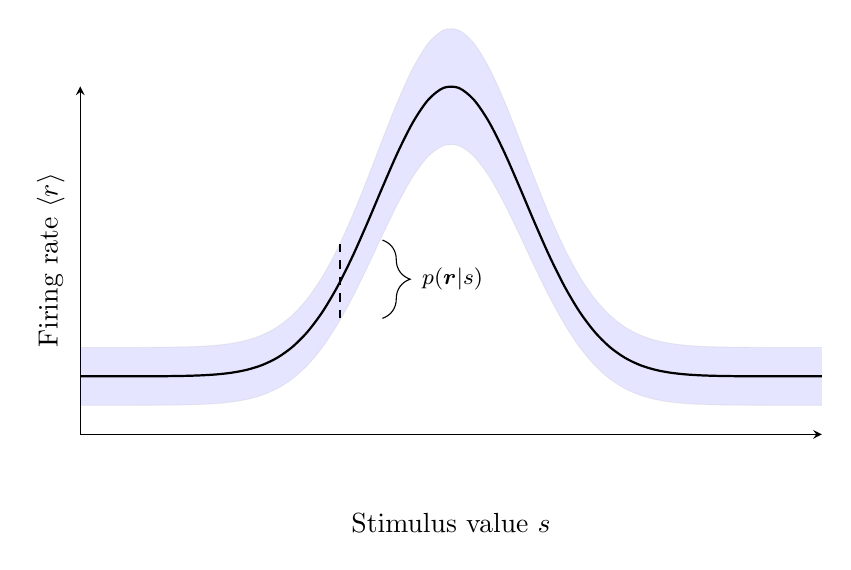
\begin{tikzpicture}
        \begin{axis}[
            width=11cm,
            height=6cm,
            xlabel={Stimulus value $s$},
            xlabel style={at={(axis description cs:0.5,-0.2)}, anchor=north},
            ylabel={Firing rate $\langle r \rangle$},
            axis y line=left,
            axis x line=bottom,
            xmin=0, xmax=10,
            ymin=-2, ymax=10,
            clip=false,
            domain=0:10,
            xtick=\empty,
            ytick=\empty
        ]
        
        % Gaussian kernel
        \addplot[
            name path=main,
            domain=0:10,
            samples=100,
            thick,
            black,
            samples=50,
            unbounded coords=jump,
            smooth
        ] {10*exp(-((x-5)^2)/(2*1^2))}; % Gaussian function with mean 5 and stddev 1

        \addplot[
            name path=top,
            domain=0:10,
            samples=100,
            thin,
            gray,
            samples=50,
            unbounded coords=jump,
            smooth,
            opacity=0.1
        ] {1+11*exp(-((x-5)^2)/(2*1^2))}; % Gaussian function with mean 5 and stddev 1

        \addplot[
            name path=bottom,
            domain=0:10,
            samples=100,
            thin,
            gray,
            samples=50,
            unbounded coords=jump,
            smooth,
            opacity=0.1
        ] {-1+9*exp(-((x-5)^2)/(2*1^2))}; % Gaussian function with mean 5 and stddev 1

        \addplot [
            thick,
            color=blue,
            fill=blue, 
            fill opacity=0.1
        ]
        fill between[
            of=top and bottom
        ];

        \addplot[
            color=black,
            dashed,
            thick
        ]
        coordinates {
            (3.5, 2) (3.5, 4.7)
        };

        \draw[decorate,decoration={brace,amplitude=10pt,mirror,raise=2pt}] 
            (axis cs:4,2) -- (axis cs:4,4.7) node[midway,xshift=10pt,right] {\footnotesize $\text{ }p(\bm{r}|s)$};

        \end{axis}
    
    \end{tikzpicture}

\end{figure}


Recall, for example, the form of the Poisson distribution, assuming independence between different neurons, and where each neuron $a$ is described by a different tuning curve $f_a(s)$:\\
\begin{equation*}
    p(\bm{r}|s) = \prod_a \frac{e^{-f_a(s)T}(f_a(s)T)^{r_aT}}{(r_aT)!}
\end{equation*}

To be very clear here, the term $f_a(s)T$ is the mean spike-count of neuron $a$ given our tuning curve, and $r_aT$ is the spike-count we actually measure.\\

\begin{figure}[H]
    \centering
    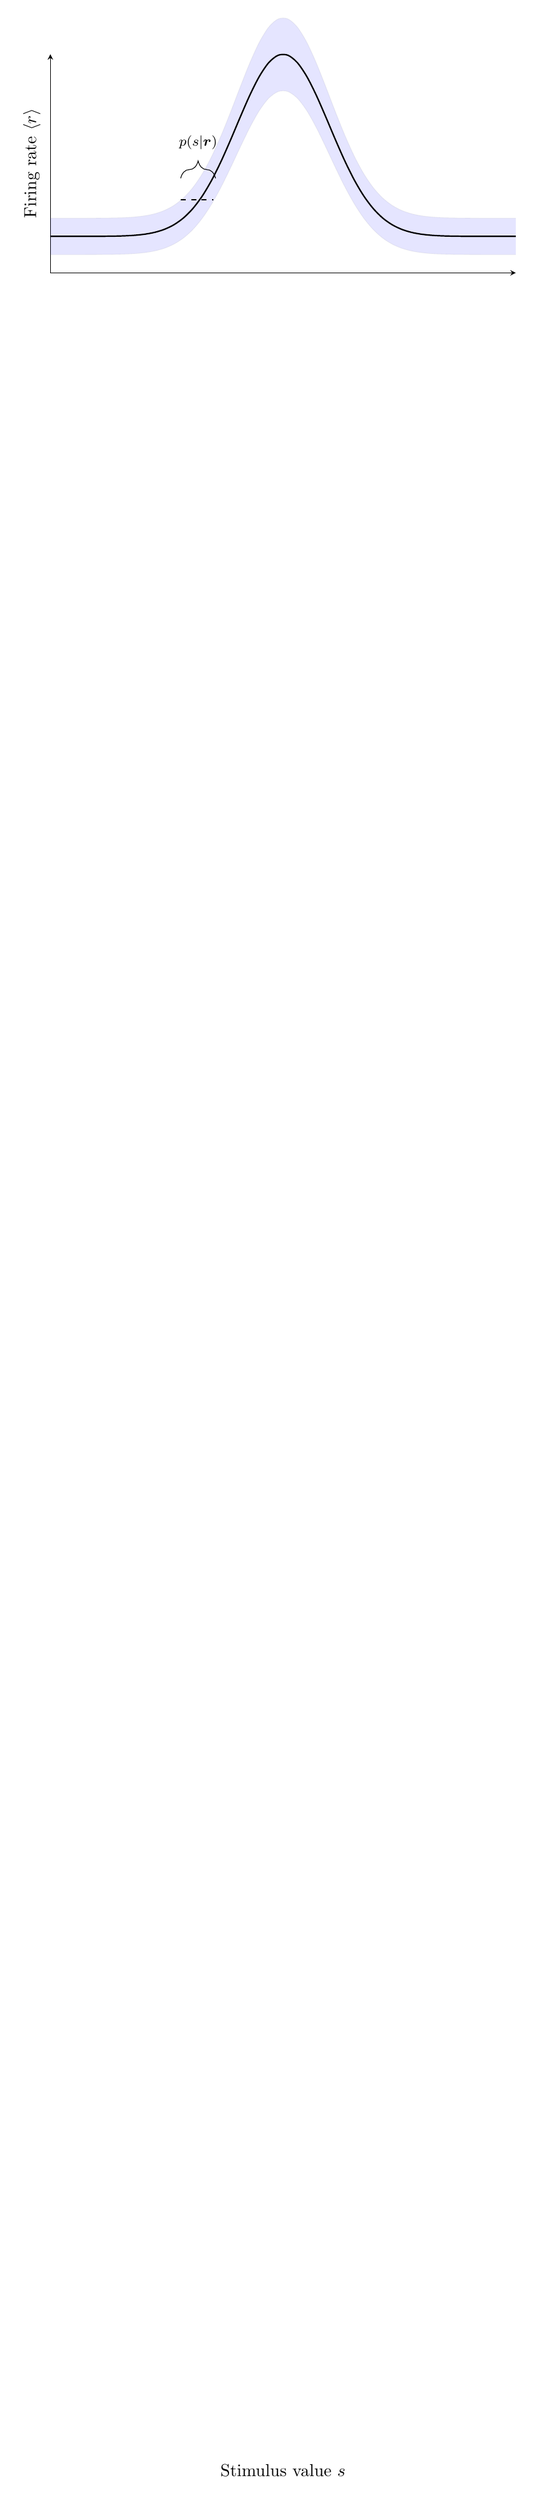
\begin{tikzpicture}
        \begin{axis}[
            width=11cm,
            height=6cm,
            xlabel={Stimulus value $s$},
            xlabel style={at={(axis description cs:0.5,-10)}, anchor=north},
            ylabel={Firing rate $\langle r \rangle$},
            axis y line=left,
            axis x line=bottom,
            xmin=0, xmax=10,
            ymin=-2, ymax=10,
            clip=false,
            domain=0:10,
            xtick=\empty,
            ytick=\empty
        ]
        
        % Gaussian kernel
        \addplot[
            name path=main,
            domain=0:10,
            samples=100,
            thick,
            black,
            samples=50,
            unbounded coords=jump,
            smooth
        ] {10*exp(-((x-5)^2)/(2*1^2))}; % Gaussian function with mean 5 and stddev 1

        \addplot[
            name path=top,
            domain=0:10,
            samples=100,
            thin,
            gray,
            samples=50,
            unbounded coords=jump,
            smooth,
            opacity=0.1
        ] {1+11*exp(-((x-5)^2)/(2*1^2))}; % Gaussian function with mean 5 and stddev 1

        \addplot[
            name path=bottom,
            domain=0:10,
            samples=100,
            thin,
            gray,
            samples=50,
            unbounded coords=jump,
            smooth,
            opacity=0.1
        ] {-1+9*exp(-((x-5)^2)/(2*1^2))}; % Gaussian function with mean 5 and stddev 1

        \addplot [
            thick,
            color=blue,
            fill=blue, 
            fill opacity=0.1
        ]
        fill between[
            of=top and bottom
        ];

        \addplot[
            color=black,
            dashed,
            thick
        ]
        coordinates {
            (2.8, 2) (3.5, 2)
        };

        \draw[decorate,decoration={brace,amplitude=10pt,raise=2pt}] 
            (axis cs:2.8,3) -- (axis cs:3.55,3)
            node[midway, above=15pt] {\footnotesize $p(s|\bm{r})$};

        \end{axis}
    
    \end{tikzpicture}

\end{figure}

So our procedure at this point is to fit the parameters of a tuning curve for each neuron to the measured data, and use this to describe a generative model that gives a distribution of firing rates for each neuron given a stimulus. Now the decoding task is to estimate the stimulus \textit{given} the firing rates. This is done using Bayes' theorem, which states that the posterior distribution of the stimulus given the firing rates is proportional to the likelihood of the firing rates given the stimulus, times the prior distribution of the stimulus:

\begin{align*}
    p(s|\bm{r}) &= \frac{p(\bm{r}|s)p(s)}{p(\bm{r})}\\[10pt]
    \text{Posterior} &= \frac{\text{Likelihood} \times \text{Prior}}{\text{Evidence}}
\end{align*}

The prior term, $p(s)$, represents our 'best guess' distribution over the stimulus values before we have any knowledge of the neural response. For example, if we know the stimulus takes value $a$ two-thirds of the time, and $b$ one-third of the time, then we could set $p(s=a)=2/3$ and $p(s=b)=1/3$. If no such information is available, then we typically set our prior to a uniform distribution, or some other distribution that is relatively uninformative - typically, for relatively sensible priors, the results won't be affected too much.\\

The evidence term is calculated by marginalising over the stimulus, and acts as a normalising constant. In full:

\begin{equation*}
    p(\bm{r}) = \int ds p(\bm{r}|s)p(s)
\end{equation*}

As we can see, dividing by this term just ensures that we have a well-defined probability distribution, as integrals over a probability distribution must be equal to 1.\\

The full Bayesian approach would be to just leave things here: given a measured neural response, we return the probability distribution over possible stimulus values given by Bayes' theorem. However, there are cases where we require a point estimate of the stimulus, ie, a specific value of $s$ that we determine to be the 'best' estimate of $s$ given $\bm{r}$. One method of doing this is to take the mode of the posterior distribution - that is, the value of $s$ that maximises the posterior distribution. This is known as MAP estimation (maximum a posteriori). It has the benefit of us not needing to calculate the normalising constant, which is typically analytically intractable, and can be computationally expensive to approximate. Note that we can plug our posterior into any monotonic (always increasing) function, and the MAP estimate will be identical. Typically, we therefore maximise the log posterior, as the logarithm function has nice algebraic properties:

\begin{equation*}
    s_{MAP} = \text{argmax}_s \log p(\bm{r}|s) + \log p(s)
\end{equation*}

And we see that we can safely ignore the $-\log p(\bm{r})$ term, as it does not depend on $s$.\\

As with many optimisation problems, the solution for many models is determined by differentiating the log posterior with respect to the stimulus, and setting the result to zero. This can give an exact analytical solution for $s_{MAP}$, into which we can plug in any firing rate vector $\bm{r}$ and get out our best estimate of the stimulus that caused it. The book covers some examples of solutions where this is the case.\\

The maximum likelihood (ML) approach is to give instead the stimulus that maximises $\log p(\bm{r}|s)$. This is identical to the MAP estimate, but ignores the prior, and is therefore equivalent to using a uniform prior that is independent of $s$.

\subsection{Fisher information}

Fisher information is a measure of how much information a neuron, or population of neurons, can carry about a stimulus. It tells us the amount of accuracy with which we can hope to decode a stimulus value. It is therefore useful in the theoretical derivation of error bounds for decoding algorithms, which are beyond the scope of these notes. However, a brief discussion of Fisher information is helpful here as it aids our understanding of how neurons encode information. Note that a somewhat more useful measure is given by Shannon's mutual information, which we will discuss in the next chapter.\\

Consider, once more, the tuning curve of a neuron. Imagine that we want to decode a stimulus value in the presence of noise. The diagram below shows the deviation of our decoding at a region where the tuning curve is steep, and a region where the tuning curve is shallow. The key takeaway from this section is that neurons are maximally informative about a stimulus at regions where their tuning curve is steepest. The diagram makes this obvious, but it may be somewhat surprising at first, as we would naively assume neurons are maximally informative where they are responding the most.

\begin{figure}[H]
    \centering
    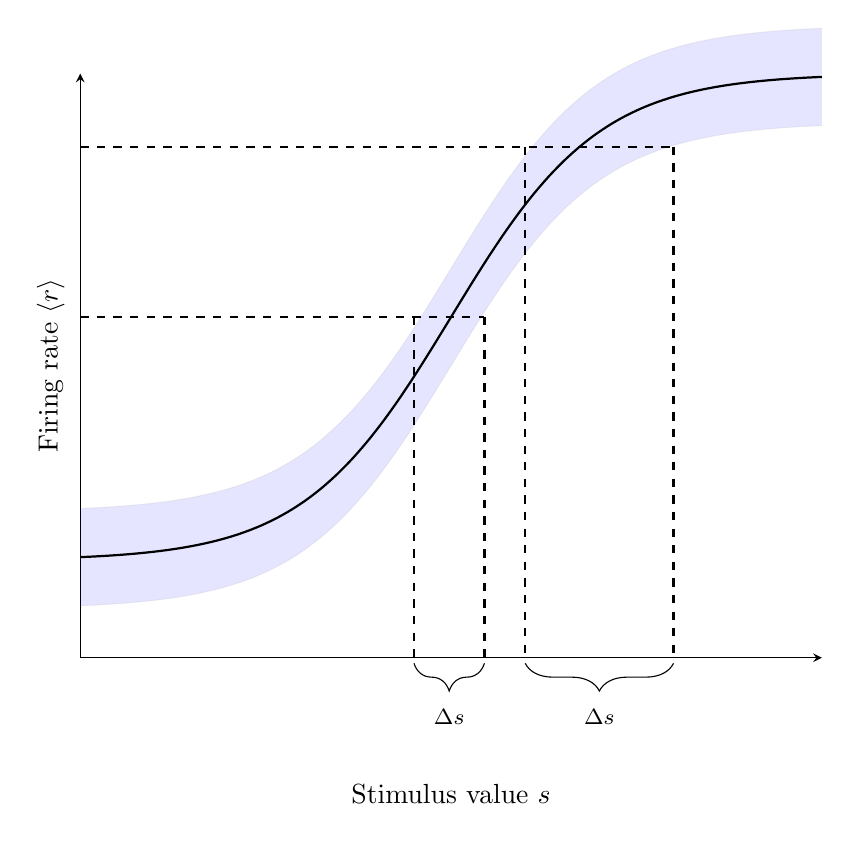
\begin{tikzpicture}
        \begin{axis}[
            width=11cm,
            height=9cm,
            xlabel={Stimulus value $s$},
            xlabel style={at={(axis description cs:0.5,-0.2)}, anchor=north},
            ylabel={Firing rate $\langle r \rangle$},
            axis y line=left,
            axis x line=bottom,
            xmin=0, xmax=10,
            ymin=-2, ymax=10,
            clip=false,
            domain=0:10,
            xtick=\empty,
            ytick=\empty
        ]
        
        % Gaussian kernel
        \addplot[
            name path=main,
            domain=0:10,
            samples=100,
            thick,
            black,
            samples=50,
            unbounded coords=jump,
            smooth
        ] {10*exp(x-5)/(1+exp(x-5)))}; % Gaussian function with mean 5 and stddev 1

        \addplot[
            name path=top,
            domain=0:10,
            samples=100,
            thin,
            gray,
            samples=50,
            unbounded coords=jump,
            smooth,
            opacity=0.1
        ] {1+10*exp(x-5)/(1+exp(x-5)))}; % Gaussian function with mean 5 and stddev 1

        \addplot[
            name path=bottom,
            domain=0:10,
            samples=100,
            thin,
            gray,
            samples=50,
            unbounded coords=jump,
            smooth,
            opacity=0.1
        ] {-1+10*exp(x-5)/(1+exp(x-5)))}; % Gaussian function with mean 5 and stddev 1

        \addplot [
            thick,
            color=blue,
            fill=blue, 
            fill opacity=0.1
        ]
        fill between[
            of=top and bottom
        ];

        \addplot[
            color=black,
            dashed,
            thick
        ]
        coordinates {
            (0,5) (5.45,5)
        };

        \addplot[
            color=black,
            dashed,
            thick
        ]
        coordinates {
            (5.45,5) (5.45,-2)
        };

        \addplot[
            color=black,
            dashed,
            thick
        ]
        coordinates {
            (4.5,5) (4.5,-2)
        };

        \draw[decorate,decoration={brace,mirror,amplitude=10pt,raise=2pt}] 
            (axis cs:4.5, -2) -- (axis cs:5.45,-2)
            node[midway, below=15pt] {\footnotesize $\Delta s$};

        \addplot[
            color=black,
            dashed,
            thick
        ]
        coordinates {
            (0,8.5) (8,8.5)
        };

        \addplot[
            color=black,
            dashed,
            thick
        ]
        coordinates {
            (6,8.5) (6,-2)
        };

        \addplot[
            color=black,
            dashed,
            thick
        ]
        coordinates {
            (8,8.5) (8,-2)
        };

        \draw[decorate,decoration={brace,mirror,amplitude=10pt,raise=2pt}] 
            (axis cs:6, -2) -- (axis cs:8,-2)
            node[midway, below=15pt] {\footnotesize $\Delta s$};

        \end{axis}
    
    \end{tikzpicture}

\end{figure}

The Fisher information captures this through the term $\left ( \frac{\partial\ln p(\bm{r}|s)}{\partial s} \right)^2$, where the square ensures that it doesn't matter if the slope is pointing up or down, and the logarithm is used for its nice algebraic properties. This is not defined for the mean of the tuning curve as shown in the diagram but for the entire conditional probability distribution, so we then just take the mean of this term over the entire set of possible responses:

\begin{equation*}
    I_F(s) = \int d\bm{r} p(\bm{r}|s)\left ( \frac{\partial\ln p(\bm{r}|s)}{\partial s} \right)^2
\end{equation*}

Plugging in a value of $s$ into the Fisher information gives us a measure of how much information the neural response can have about the stimulus at that point.

\subsection{Spike-train decoding}

So far, we have only considered rate-based decoding methods. If we want to decode a time-varying stimulus, then we need to use spike-trains. A basic statement of this problem is that we are given as input a series of spike-times $(t_1,...,t_n)$ up to a time $t$, and we want to predict the stimulus value at this time, $s(t)$. Recall that we often describe a spike-train using a sum of dirac-delta functions to give a continuous function $\rho (\tau)$. In the diagram below, note that $\tau$ is the time parameter we use to describe the history of the trial so far, which we can use to predict the stimulus at the current time point $t$.\\

\begin{figure}[H]
    \centering
    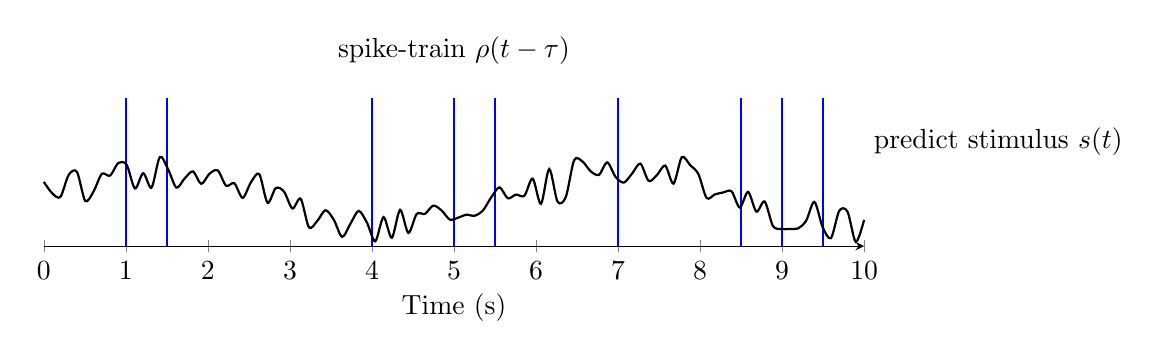
\begin{tikzpicture}
        % Define some colors for the stimulus and STA window
        \definecolor{stimuluscolor}{RGB}{150, 150, 255}
        \definecolor{stawindowcolor}{RGB}{255, 200, 200}
        
        \begin{axis}[
            width=12cm,
            height=4cm,
            xlabel={Time (s)},
            xlabel style={at={(axis description cs:0.5,-0.2)}, anchor=north},
            axis y line=none,
            axis x line=bottom,
            xmin=0, xmax=10,
            ymin=0, ymax=2,
            clip=false,
            domain=0:10
        ]

        % Spike train for a single neuron (small vertical lines)
        \addplot+[ycomb, thick, mark=|, mark size=2pt, color=blue] 
            coordinates {
                (1, 1.5)
                (1.5, 1.5)
                (4, 1.5)
                (5, 1.5)
                (5.5, 1.5)
                (7, 1.5)
                (8.5, 1.5)
                (9, 1.5)
                (9.5, 1.5)
            };

        \addplot[
            domain=0:10,
            samples=100,
            thick,
            black,
            smooth
        ] {0.5 + 0.3 * sin(2*pi*10*x) + 0.2 * rand};

        \node[anchor=west] at (axis cs:10, 1.1) {predict stimulus $s(t)$};
        \node[anchor=north] at (axis cs:5, 2.3) {spike-train $\rho (t-\tau)$};

        \end{axis}
    \end{tikzpicture}

\end{figure}

This problem is in fact almost exactly the reverse of the time-varying neural encoding problem we met in chapter 2. However, there are a couple of crucial differences that warrant discussion. As we've already discussed, in a laboratory setting, we can treat the stimulus as an independent variable, which causes the dependent variable that is the neural response. This means we can give the stimulus any structure we want, such as making it a white noise stimulus, which is how we solved the encoding problem. When decoding, however, we can't directly control the neural response, so we have to work with whatever response we are given. Furthermore, in the time-varying case, the direction of causation makes our problem statement quite unusual: the stimulus causes future values of the response, yet we are trying to predict the stimulus from the response's history. This is, of course, only possible if the history of the \textit{stimulus} provides information about the future stimulus, as the neural response can in reality only tell us about the stimulus that caused it, not the future stimulus.\\

\begin{figure}[H]
\centering
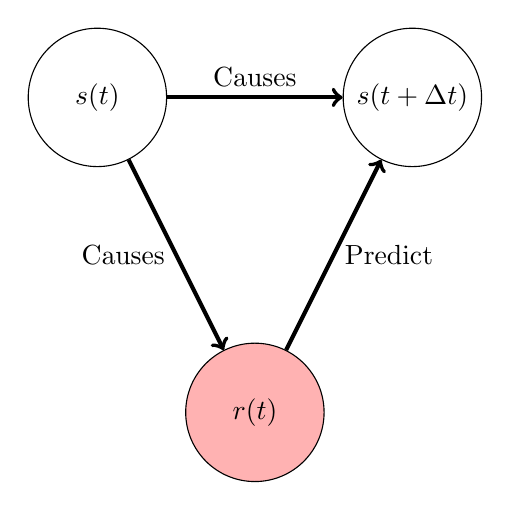
\begin{tikzpicture}
    % Define a style for all nodes
    \tikzstyle{node} = [draw, circle, minimum size=50pt, inner sep=0pt]

    % Nodes
    \node[node] (s) at (0, 4) {$s(t)$};
    \node[node] (s') at (4, 4) {$s(t+\Delta t)$};
    \node[node, fill=red!30] (r) at (2, 0) {$r(t)$}; % Different color for r

    % Edges with arrows
    \draw[->, line width=1.5pt] (s) -- node [midway, left] {Causes} (r);
    \draw[->, line width=1.5pt] (r) -- node [midway, right] {Predict} (s');
    \draw[->, line width=1.5pt] (s) -- node [midway, above] {Causes} (s');
\end{tikzpicture}
\end{figure}

In the diagram above, we can only observe the response, but can use this to predict the stimulus at a later time, as they are still correlated via the stimulus history. This does mean, however, that spike-train decoding is impossible if the stimulus is white-noise: we require internal structure within the stimulus.\\

A classic application of spike-train decoding methods would be a brain-computer interface, where we are trying to gain information about a stimulus on the fly from neural activity. For this reason, we talk about spike-train decoding, rather than firing rate decoding: we want to be able to form a prediction for a single trial, as we won't necessarily be able to record many trials to smooth over to give the firing rate function. Additionally, note that we introduce a time lag $\tau_0$ into our decoding, as this increases accuracy, as it allows \textit{some} spikes to occur after the stimulus we are decoding, and therefore be casued by them. However, too large a time lag would make many BCI applications impossible.\\

Proceeding exactly like the encoding case, we want to form a linear estimate of the stimulus at time $t-\tau_0$, given the entire spike-train up to the time $t$. This is done by integrating over the whole trial with a kernel $K(\tau)$. Note in the equation shown, the integral is over all time, not from time 0 to infinity as you might expect. This means technically we are considering spikes after the time $t$ (recall $\tau$ runs backwards from time $t$). This can be avoided by making the kernel acausal, which means we clamp its value to 0 for negative values of $\tau$.

\begin{equation*}
    s_{est}(t-\tau_0) = \int_{-\infty}^\infty d\tau (\rho(t-\tau)-\langle r \rangle)K(\tau)
\end{equation*}

Our job is to figure out the kernel that gives the \textit{best} estimate of the stimulus given the spike-train. Just like with neural encoding, we consider a training set of trials where we measure both the spike-trains and the stimulus, and minimise the following mean squared error over all these trials:

\begin{equation*}
    \text{MSE} = \frac{1}{T}\int_0^T dt \left\langle \left ( s(t-\tau_0) - s_{est}(t-\tau_0) \right)^2\right\rangle
\end{equation*}

We can't minimise this like before, because the neural response is not white noise (it has a non-delta autocorrelation), so the full solution requires a Fourier decomposition which is beyond the scope of these notes. However, in the case of a low firing rate, where effects such as the refractory period don't matter much, our spike-trains effectively have zero auto-correlation and the solution is very interpretable, so we briefly mention what the solution amounts to.\\

Recall the spike-triggered average $C(\tau)$ discussed in chapter 1. Our optimal kernel amounts to the spike-triggered average, defined so that we consider stimuli after spikes rather than before, and shifted an amount $\tau_0$ to the left, to account for the time lag. Our decoding procedure then just sums up the spike-triggered average over all spikes, as shown in the figure below.\\

\begin{figure}[h]
    \centering
    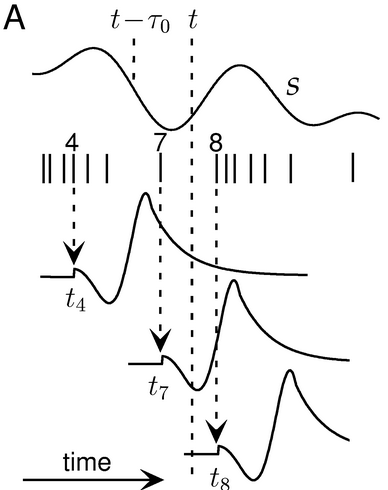
\includegraphics[width=0.5\textwidth]{decoding.png} % Adjust the width as needed
    \label{fig:example_png}
\end{figure}

This is in fact an extremely intuitive result. If we only measured one spike, our best possible guess for the stimulus' future values would be the spike-triggered average following this spike. In the presence of many spikes, we do the same thing, summing over the best possible guess provided by each spike individually.

\end{document}
